\subsubsubsubsection{Parser}
\begin{figure}[h]
\centering
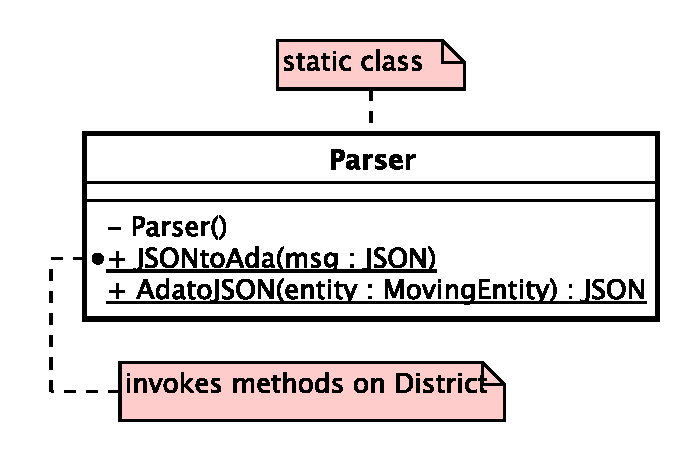
\includegraphics[scale=0.6,keepaspectratio]{images/solution/parser.eps}
\caption{\pInterface::Parser}
\label{fig:sd-app-parser}
\end{figure}
\FloatBarrier
\begin{itemize}
  \item \textbf{\descr} \\
    It represents a parser which converts JSON messages to Ada statements and vice versa.
    It is a static class because it is composed of only static methods.
  \item \textbf{\ops}
  \begin{itemize}
   \item[-] \texttt{Parser()} \\
   Private and unique constructor because \texttt{Parse} provides only static methods 
   so there are no reasons a client creates instances of \texttt{Parse}.
    \item[+] \texttt{\underline{JSONtoAda(msg: JSON)}} \\
    Converts the JSON message to Ada statements invoking district.
    \item[+] \texttt{\underline{AdatoJSON(entity: MovingEntity) : JSON}} \\
    Converts a moving entity into a JSON message returning the message as result.
  \end{itemize}
\end{itemize}
